\documentclass{article}
\usepackage[utf8]{inputenc}
\usepackage[inner=3.5cm,outer=3.5cm,top=3.0cm,bottom=3.0cm]{geometry}
\usepackage{graphicx}
\usepackage{subcaption}

\title{Machine Learning Miniproject 1}
\author{Diogo Cosin and Ralph Florent}
\date{16.March.2019}

\begin{document}

\maketitle

\section{Task Description}

The project is a programming exercise that requires to code the K-means clustering Machine Learning algorithm. Once implemented, the coded algorithm should be able to regroup into K(1, 2, 3, 200) clusters of digit images from the "Optical Character Recognition (OCR)" dataset provided by Prof. Dr. H. Jaeger. Additionally, a few examples of visualizations of the obtained results should be provided as well as the respective analysis of the results.

\section{Results Obtained and Analysis}

The K-means algorithm implemented is executed different times to check its behavior with varying values of K. In this section, we visualize the results obtained and discuss them.

\subsection{Execution with One Single Cluster}

We begin our analysis by setting the number of clusters K to 1 and applying the created K-means algorithm to the "sevens" digits in the OCR dataset, and this means 240 samples in total.

In this scenario, the K-means algorithm should allocate all data points into a single cluster. Practically speaking, this will not produce any relevant results, as this is no different of working with the whole dataset.

After executing K-means algorithm in the previously described condition, it is obtained the codebook vector whose image is represented in Figure \ref{fig:codebook1}.

\begin{figure}[h!]
    \centering
    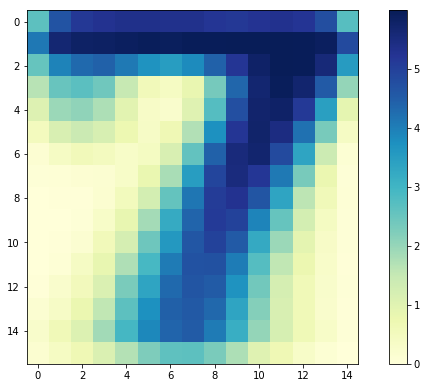
\includegraphics[scale=0.4]{images/codebook_cluster1.png}
    \caption{Codebook Vector Image for K=1.}
    \label{fig:codebook1}
\end{figure}

Figure \ref{fig:codebook1} shows what would the average "seven" digit in the OCR dataset, as the codebook vector, in this case, is the mean of all data points in the dataset. Clearly, most data points have a "traditional" seven format. For this reason, the pixels corresponding to the positions of a "traditional" seven are represented in darker color, while the lighter pixels and more blurry regions are related to regions not clearly standardized in a typical seven drawing in the OCR dataset.

\subsection{Execution with Two Clusters}

Carrying on with the clustering analysis, we now turn our attention to the case whose number of clusters is set to 2. In this case, the K-means algorithm will arrange the data points into two clusters, unless in the rare case where one of them becomes empty during the convergence process.

Executing the K-means algorithm for K=2, lead us to the codebook vector images showed in Figure \ref{fig:codebook2}.

\begin{figure}[h!]
    \centering
    \begin{subfigure}[b]{0.4\linewidth}
      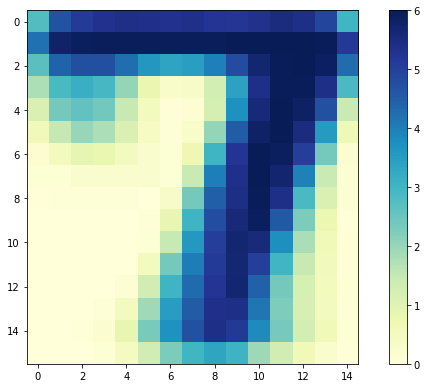
\includegraphics[scale=0.4]{images/codebook_cluster2_1.png}
      \caption{Cluster 1.}
    \end{subfigure}\hspace{20.0}%
    \begin{subfigure}[b]{0.4\linewidth}
      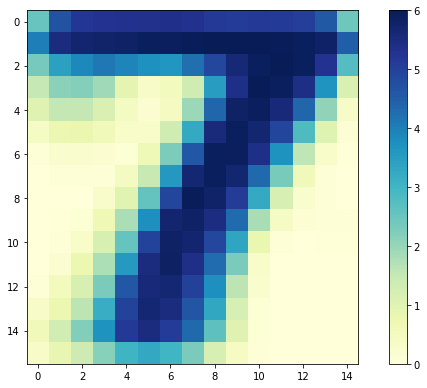
\includegraphics[scale=0.4]{images/codebook_cluster2_2.png}
      \caption{Cluster 2.}
    \end{subfigure}
    \caption{Codebook Vector Images for K=2.}
    \label{fig:codebook2}
\end{figure}

Now, with two clusters, it is possible to notice that the blurry regions (transition between the light and dark pixels) in the codebook vectors images decreased when compared to the codebook vector of the single cluster, as showed in Figure \ref{fig:codebook1}.

This behavior was already to be expected, given that using more clusters. There will be a better separation of the data points. That is, similar data points will be allocated in the same cluster and, consequently, the mean digit of that cluster, the codebook vector, will be better defined.

\subsection{Execution with Three Clusters}

Similarly, we execute the K-means algorithm for K=3. The codebook vectors obtained in this case have their image represented in Figure \ref{fig:codebook3}.

\begin{figure}[h!]
    \centering
    \begin{subfigure}[b]{0.4\linewidth}
      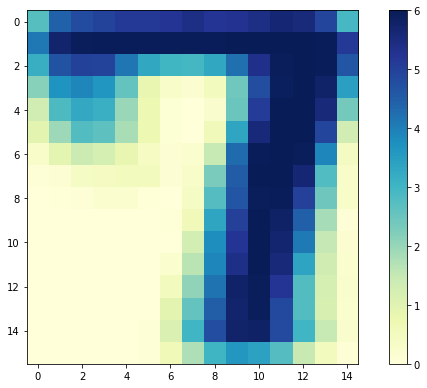
\includegraphics[scale=0.4]{images/codebook_cluster3_1.png}
      \caption{Cluster 1.}
    \end{subfigure}\hspace{20.0}%
      \begin{subfigure}[b]{0.4\linewidth}
      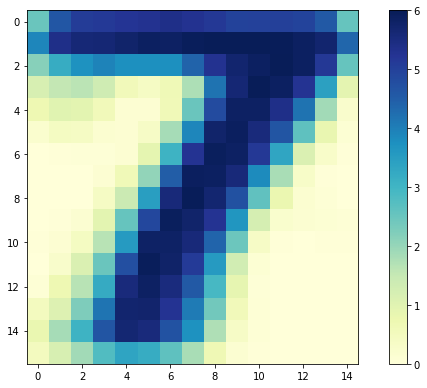
\includegraphics[scale=0.4]{images/codebook_cluster3_2.png}
      \caption{Cluster 2.}
    \end{subfigure}\\[1ex]
    \begin{subfigure}[b]{0.4\linewidth}
      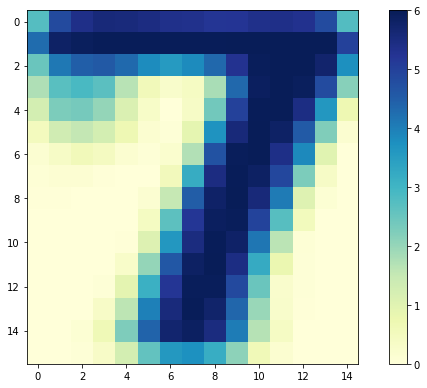
\includegraphics[scale=0.4]{images/codebook_cluster3_3.png}
      \caption{Cluster 3.}
    \end{subfigure}
    \caption{Codebook Vector Images for K=3.}
    \label{fig:codebook3}
\end{figure}

Following the trend already observed for the two-cluster case showed in Figure \ref{fig:codebook2}, increasing the number of clusters makes the codebook vectors images more consistent with less blurry regions.

\subsection{Execution with 200 Clusters}

Finally, we follow the case where K is set to 200. In this scenario we expect that most clusters will have only one data point, considering that the OCR dataset provides 240 samples for each digit.

Figure \ref{fig:codebook200} shows 4 out of the 199 codebook vectors obtained setting K=200. It was obtained 199 clusters instead of 200 because two samples were  the same and ended up being allocated to the same cluster. This way, one extra cluster was discarded.

\begin{figure}[h!]
    \centering
    \begin{subfigure}[b]{0.4\linewidth}
      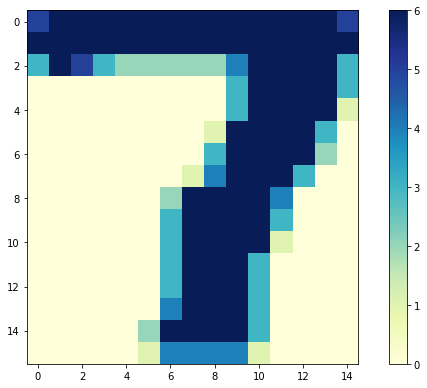
\includegraphics[scale=0.4]{images/codebook_cluster4_1.png}
      \caption{Cluster 1.}
    \end{subfigure}\hspace{20.0}%
      \begin{subfigure}[b]{0.4\linewidth}
      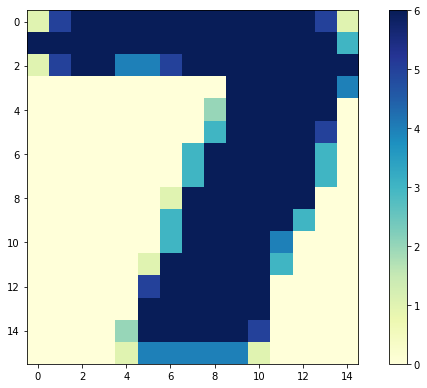
\includegraphics[scale=0.4]{images/codebook_cluster4_2.png}
      \caption{Cluster 2.}
    \end{subfigure}\\[1ex]
    \begin{subfigure}[b]{0.4\linewidth}
      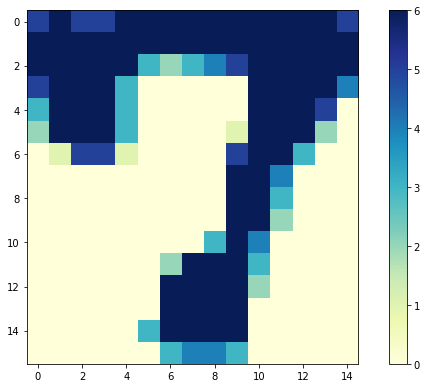
\includegraphics[scale=0.4]{images/codebook_cluster4_3.png}
      \caption{Cluster 3.}
    \end{subfigure}\hspace{20.0}%
    \begin{subfigure}[b]{0.4\linewidth}
      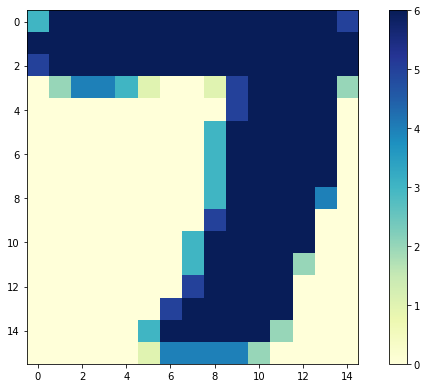
\includegraphics[scale=0.4]{images/codebook_cluster4_4.png}
      \caption{Cluster 4.}
    \end{subfigure}
    \caption{Codebook Vector Images for K=200. Only four of them are shown.}
    \label{fig:codebook200}
\end{figure}

Each codebook vector is the image of the single digit allocated to it. Still, some clusters received two identical data points, but as they are the same, the practical effect on the codebook vector is the same as if there was only one data point in the cluster.

Figure \ref{fig:codebook200} shows that codebook vector images present insignificant blurry regions; the transitions are still present due to the image nature itself and not because of the variance among samples in the same cluster. Setting K to 200 has the practical effect of making each digit belong to your own little cluster alone. While it can be discussed if this strategy is wise for a clustering or dimension reduction task, it cannot be discussed its efficiency when the objective is to allocate each sample to the most similar cluster possible.

\subsection{Mathematical Nature of the Codebook Image When K=1}

When the K-means algorithm is run for K=1 over the dataset, the output results in one cluster, as Figure \ref{fig:codebook1} shows, which contains all the data points of the dataset. Then, intuitively speaking, the codebook vector image becomes the mean of the data points being part of the single cluster. Therefore, the mathematical nature that can be deduced from this remark can be expressed as follows:

\begin{equation}
 For K = 1, c_{1} = \frac{1}{N} \cdot \sum_{i=1}^N x_{i}
\end{equation}
where $N$ is the number of samples applied to the K-means algorithm, $c_{1}$, the codebook vector, and $x_{i}$ are the data points.

\subsection{Mathematical Nature of the Codebook Image When K=200}

For K=200, which is, by the way, the same size as the digit-pattern subset, the K-means algorithm will output 200 (not the case for every digit, 7 for example) clusters, where each cluster has a single data point (vector image) of the digit-pattern subset. In other words, every cluster has one data point that in turn serves as the corresponding codebook vector for this particular cluster. Consequently, we can express the mathematical nature of such a description by:

\begin{equation}
 For K = 200, c_{i} =  x_{i}
\end{equation}
where $c_{i}$ are the codebook vectors for the 200 clusters, and $x_{i}$ are the data points belonging to each cluster.

\subsection{Clustering Several Digits}

In this subsection, instead of applying the K-means algorithm directly to single digit data, like it has been previously done with the "seven" digit data, we apply the very same algorithm to a more diverse dataset. This time, samples from all the classes (0 to 9) are selected and applied to the K-means algorithm. The dataset is programmatically built in a way to contain 20 samples of each class, totalizing 200 samples as shown in Figure \ref{fig:several_dataset}.

\begin{figure}[h!]
    \centering
    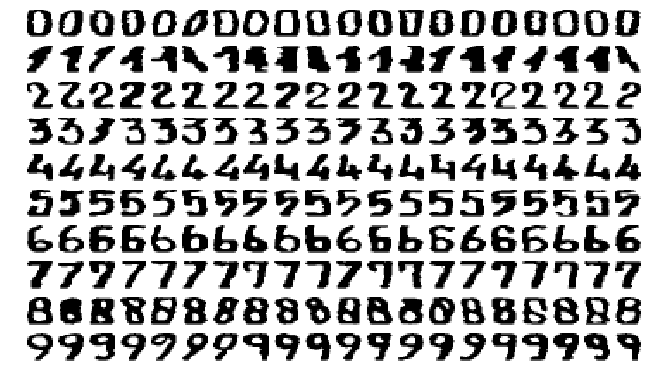
\includegraphics[width=\textwidth]{images/dataset_several_digits.png}
    \caption{Dataset with several digits.}
    \label{fig:several_dataset}
\end{figure}

We then apply this dataset to the K-means algorithm setting K=20. In this scenario, it is possible to get interesting insights from how data points of different digits may relate to each other. For instance, Figure \ref{fig:5_among_3} shows that a given five-digit sample is similar to some samples of the three-digit class.

\begin{figure}[h!]
    \centering
    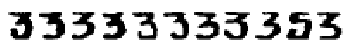
\includegraphics[width=\textwidth]{images/5_among_3s.png}
    \caption{A 5 sample clustered among 3s samples.}
    \label{fig:5_among_3}
\end{figure}

This insight may be important if in the future we try to build a classifier to this dataset. In this case, we may have problems distinguishing some fives-digit samples from threes-digit samples.

Another interesting insight is that some eights may be confused with zeros. For instance, Figure \ref{fig:8_among_0} shows this particular situation. 

\begin{figure}[h!]
    \centering
    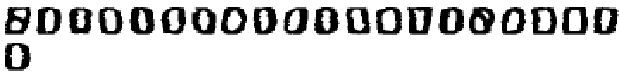
\includegraphics[width=\textwidth]{images/8_among_0s.png}
    \caption{A 8 sample clustered among 0s samples.}
    \label{fig:8_among_0}
\end{figure}

As in the case showed in Figure \ref{fig:5_among_3}, this similarity between this specific eight and the zeros may be a hurdle when fitting a classifier for the digits.

Other interesting insights are observed, but to avoid making this report longer than expected, we summarize them in a single image, shown in Figure \ref{fig:remaining_example}.

\begin{figure}[h!]
    \centering
    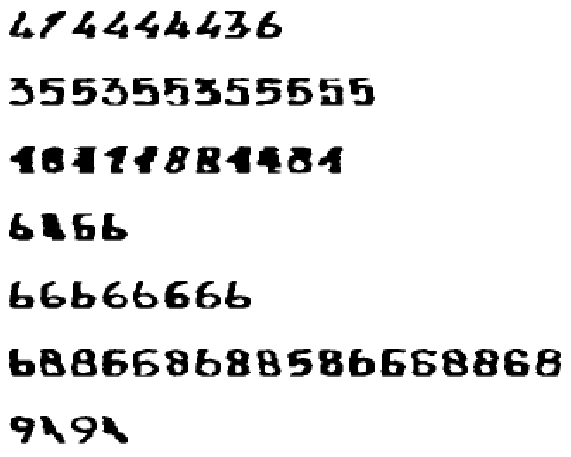
\includegraphics[scale=0.51]{images/remaining_examples.png}
    \caption{A 8 sample clustered among 0s samples.}
    \label{fig:remaining_example}
\end{figure}

\section{Conclusion}

Observing the results by running the K-mean clustering on the mixed digit-class pattern dataset, we notice that the digits that share certain similarities, such as slightly tilted to the left or the right, tend to cluster together.

More interestingly, certain digits like zero, five, six, eight, and nine are really close in terms of shape. That is, given a digit-pattern from the mentioned set, a classifier might misclassify the class-digit. For instance, the digit-pattern might have the shape of a five, and the output results in an eight when the true value is a six. That's a closely-alike shape issue.

Also when we run the K-means algorithm for K = 20, we observe from the visualizations that based on the closely-alike shape issue mentioned above, digits like seven, zeros, and four are hardly misclassified. However, pair digits like six-eight, seven-nine for example, share certain similarities in the ending tail. That can also constitute a huge headache for the classifier.

\end{document}
